\documentclass{article}

\usepackage{tikz}
\usepackage{amsmath}
\usepackage{amsfonts}
\usepackage{pgfplots}

\pgfplotsset{compat=1.11}
\pgfplotstableread[col sep = comma]{data/lake-cycles.csv}\mydata
\pgfplotstableread[col sep = comma]{data/six-lakes-no-purification.csv}\sixlakesnopurification
\pgfplotstableread[col sep = comma]{data/six-lakes-purification.csv}\sixlakespurification
\begin{document}

\section{Reservoir}

\subsection{Problem Statement}

In this section, I model a lake system with concentrations of a chemical.
There are $n$ lakes, which each have volume $V_i$ (see Figure \ref{fig:lakes}).
Each lake has a concentration $c_i$.

\begin{figure}[h!]
\centering
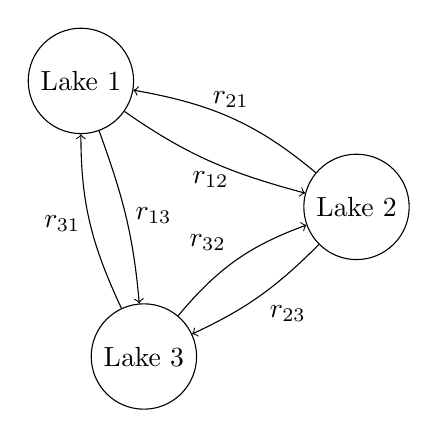
\begin{tikzpicture}

\node[draw, circle] (lake1) at (-1.3,2.2) {Lake 1};
\node[draw, circle] (lake2) at (2.2,0.6) {Lake 2};
\node[draw, circle] (lake3) at (-0.5, -1.3) {Lake 3};
\draw[<-] (lake1) to [out=-10, in=140] node[black, above] {$r_{21}$} (lake2) ;
\draw[->] (lake1) to [out=-35, in=165] node[black, below] {$r_{12}$}(lake2);
\draw[->] (lake1) to [out=-70, in=95] node[black, right] {$r_{13}$} (lake3);
\draw[<-] (lake1) to [out=-90, in=115] node[black, left] {$r_{31}$} (lake3);
\draw[->] (lake3) to [out=50, in=200] node[black, above left] {$r_{32}$} (lake2);
\draw[<-] (lake3) to [out=25, in=225] node[black, below right] {$r_{23}$} (lake2);

\end{tikzpicture}
\caption{A Lake System, with flow rates}
\label{fig:lakes}
\end{figure}

The rate of flow between lake $i$ and lake $j$ is given by the difference in their
	concentrations times the rate of flow.
So, the flow into any one lake is given by the following matrix:

\begin{align}
R & = \left[ \begin{matrix}
	- \left( r_{21} + r_{31} \right) & r_{21} & r_{31} \\
	r_{12} & - \left( r_{12} + r_{32} \right) & r_{32} \\
	r_{13} & r_{23} & - \left( r_{23} + r_{13} \right) \\
\end{matrix} \right] \label{eq:def-of-R} 
\end{align}

If $C$ is a vector of concentrations, the model predicts the following flow rates:

\begin{align}
\frac{dC}{dt} & = R C \label{eq:dCdt}
\end{align}

\subsection{Asymptotic Concentrations}

We ask the question, what will the asymptotic concentrations be?
Since the system of differential equations is linear, we can solve it
	eigenvector-by-eigenvector.

We can get some insight by analyzing the eigenvalues of $R$.
Consider the following eigenvector:

\begin{align*}
\left[ \begin{matrix}
	- \left( r_{21} + r_{31} \right) & r_{21} & r_{31} \\
	r_{12} & - \left( r_{12} + r_{32} \right) & r_{32} \\
	r_{13} & r_{23} & - \left( r_{23} + r_{13} \right) 
\end{matrix} \right]
\left[ \begin{matrix} 1 \\ 1 \\ 1 \end{matrix} \right]
& = \left[ \begin{matrix} 
	r_{21} + r_{31} - \left( r_{21} + r_{31} \right) \\
	r_{12} + r_{32} - \left( r_{12} + r_{32} \right) \\
	r_{23} + r_{13} - \left( r_{23} + r_{13} \right) 
\end{matrix} \right]
& = \left[ \begin{matrix} 0 \\ 0 \\ 0 \end{matrix} \right]
\end{align*}

The vector $\left[ 0, 0, 0 \right]^T$ is an eigenvector with 
	eigenvalue zero.
If there are positive eigenvalues of $R$, then there will not
	be asymptotic concentrations, because as time goes to infinity,
	those eigenvectors will blow up in magnitude.
Therefore, it is only meaningful to talk about asymptotic concentrations
	if there are no positive eigenvalues.

As time goes to infinity, every negative eigenvalue will
	see its corresponding eigenvector's magnitude decrease to zero.
Therefore, only eigenvalues which have no negative real part will
	survive going to infinity.

The eigenvector $\left[ 1,1,1 \right]^T$ is one such eigenvector,
	with eigenvalue zero.
This eigenvector will always be present.
However, depending on the values of $r_{ij}$, there may be other 
	eigenvectors with eigenvalues with zero real part.
Only if $\left[ 1,1,1 \right]^T$ is the only eigenvector with eigenvalue 
	of real part equal to zero will generic choices of initial concentrations
	converge to a constant concentration accross the lakes.

%	\subsubsection{Example}
%	
%	The provided example in the second matlab file has the following $R$ matrix 
%		and $c_0$ initial condition vector:
%	
%	\begin{align}
%	R & = \left[ \begin{matrix}
%	-0.01 & 0 & 0 & 0 & 0 & 0.01 \\
%	0.01 & -0.01 & 0 & 0 & 0 & 0 \\
%	0 & 0.01 & -0.01 & 0 & 0 & 0 \\
%	0 & 0 & 0.01 & -0.01 & 0 & 0 \\
%	0 & 0 & 0 & 0.01 & -0.01 & 0 \\
%	0 & 0 & 0 & 0 & 0.01 & -0.01 \\
%	\end{matrix} \right] \label{eq:R-1.1} \\
%	c_0 & = \left[ \begin{matrix} 1 & 0 & 1 & 0 & 0 & 0 \end{matrix} \right]
%		\label{eq:c_0-1.1}
%	\end{align}

\subsection{Monotonicity of Convergence}

We next ask the question, will the concentrations converge monotonically
	to their final values?
This will happen if there is no cyclic behavior.
Cyclic behavior might happen in a three-reservoir system if the system
	is closely approximated by a cycle, with much larger flow
	rates in one direction than the other.
One such cycle is shown in Figure \ref{fig:lakes-with-cycle}.
Intuitively, if a large amount of the substance is dumped in one of the 
	lakes, most of the substance will make a circuit around the lakes.
The concentration might rise and fall in each reservoir until it settles down.

\begin{figure}[h!]
\centering
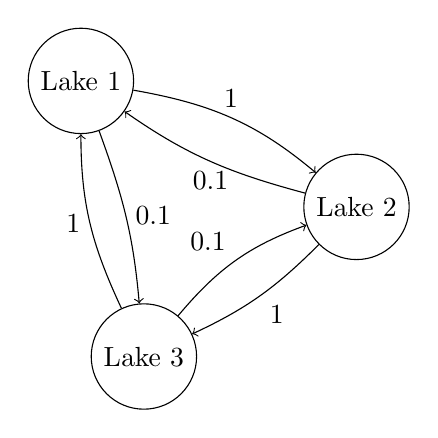
\begin{tikzpicture}

\node[draw, circle] (lake1) at (-1.3,2.2) {Lake 1};
\node[draw, circle] (lake2) at (2.2,0.6) {Lake 2};
\node[draw, circle] (lake3) at (-0.5, -1.3) {Lake 3};
\draw[<-] (lake1) to [out=-35, in=165] node[black, below] {$0.1$} (lake2) ;
\draw[->] (lake1) to [out=-10, in=140] node[black, above] {$1$} (lake2);
\draw[->] (lake1) to [out=-70, in=95] node[black, right] {$0.1$} (lake3);
\draw[<-] (lake1) to [out=-90, in=115] node[black, left] {$1$} (lake3);
\draw[->] (lake3) to [out=50, in=200] node[black, above left] {$0.1$} (lake2);
\draw[<-] (lake3) to [out=25, in=225] node[black, below right] {$1$} (lake2);

\end{tikzpicture}
\caption{A Lake System, with cyclic flow dominating}
\label{fig:lakes-with-cycle}
\end{figure}

In this case, the $R$ matrix is:

\begin{align*}
R & = \left[ \begin{matrix}
	- 1.1 & 0.1 & 1 \\
	1 & - 1.1 & 0.1 \\
	0.1 & 1 & - 1.1 \\
\end{matrix} \right] 
\end{align*}

which has eigenvalues $\lambda_1 = 0, \lambda_2 = -1.65 + 0.77942i, \lambda_3 = -1.65 - 0.77942i$
	and eigenvectors:

\begin{align*}
\lambda_1 & = 0 
	& v_1 & = \left[ \begin{matrix} 1 \\ 1 \\ 1 \end{matrix} \right] \\
\lambda_2 & = -1.65 + 0.77942i 
	& v_2 & = \left[ \begin{matrix} -0.28868 - 0.5i \\ -0.28868 + 0.5i \\ 0.57735 \end{matrix} \right] \\
\lambda_3 & = -1.65 - 0.77942i
	& v_3 & = \left[ \begin{matrix} -0.28868 + 0.5i \\ -0.28868 - 0.5i \\ 0.57735 \end{matrix} \right] \\
\end{align*}

Notice that these eigenvalues are \emph{complex}.
The answers will still be real, because they and their eigenvectors are complex
	conjugates of each other, and thus add to a real number, but their complex-ness
	can lead to the non-monotone behavior that intuition has predicted.

\begin{figure}[h!]
\centering
\begin{tikzpicture}
	\begin{axis}[
		legend pos = north east,
		xmin = 0,
		xmax = 6,
		ymin = 0,
		ymax = 1.3,
		ylabel = {$C(t)$ (units of concentration)},
		xlabel = {$t$}
	]
%	\foreach \index in {1, ..., 3} {%
%		\addplot[mark=""] table[x index = {0}, y index = {\index}]{\mydata};
%	}
	\addplot[dashed] table[x index = {0}, y index = {1}]{\mydata};
	\addlegendentry{Reservoir 1};
	\addplot[] table[x index = {0}, y index = {2}]{\mydata};
	\addlegendentry{Reservoir 2};
	\addplot[dotted] table[x index = {0}, y index = {3}]{\mydata};
	\addlegendentry{Reservoir 3};
	\end{axis}
\end{tikzpicture}
\caption{Substance Concentrations, in lake system from Figure \ref{fig:lakes-with-cycle}}
\label{fig:dynamics-with-cycle}
\end{figure}

In Figure \ref{fig:dynamics-with-cycle}, the Reservoir 2's trajectory goes above
	the equilibrium value, and then relaxes to it.
The concentration in each of the lakes is therefore not monotonic.

I conjecture that the flow in the lake with the highest initial concentration is monotonic.

\subsection{Monotonicity of Convergence in Lakes with Symmetric Flow}

\begin{figure}[h!]
\centering
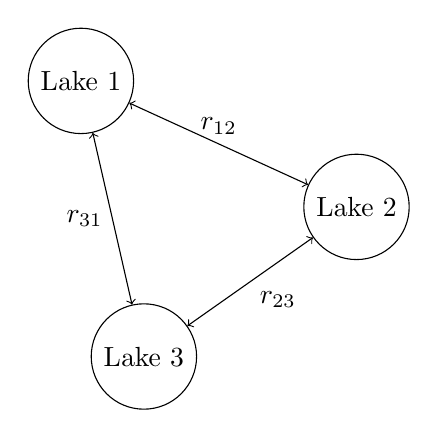
\begin{tikzpicture}

\node[draw, circle] (lake1) at (-1.3,2.2) {Lake 1};
\node[draw, circle] (lake2) at (2.2,0.6) {Lake 2};
\node[draw, circle] (lake3) at (-0.5, -1.3) {Lake 3};
\draw[<->] (lake1) to node[black, above] {$r_{12}$} (lake2) ;
\draw[<->] (lake1) to node[black, left] {$r_{31}$} (lake3);
\draw[<->] (lake3) to node[black, below right] {$r_{23}$} (lake2);

\end{tikzpicture}
\caption{A Lake System, with symmetric flow rates}
\label{fig:lakes-symmetric}
\end{figure}

Suppose we have a lake system where the rates of flow between lakes are the same
	in both directions (Figure \ref{fig:lakes-symmetric}).
Then, the $R$ matrix is symmetric.
Since symmetric matrices have real eigenvalues, then there will be no cyclic behavior.
The concentration will therefore converge monotonically in this special case.

\subsection{Water Purifying Plants}

Suppose there is a water purifying plant in lake $i$.
This plant will purify the water at a rate $\alpha_i$. 
This will add negative terms to the diagonal of the $R$-matrix:

\begin{align}
R & = \left[ \begin{matrix}
	- \left( r_{21} + r_{31} \right) - \alpha_1 & r_{21} & r_{31} \\
	r_{12} & - \left( r_{12} + r_{32} \right) - \alpha_2 & r_{32} \\
	r_{13} & r_{23} & - \left( r_{23} + r_{13} \right) - \alpha_3 \\
\end{matrix} \right] \label{eq:R-with-purification} 
\end{align}

Notice that $\left[ 1, 1, 1 \right]^T$ is no longer an eigenvector of the $R$-matrix.
Since we have assumed that there is an equilibrium limit, the eigenvalues of $R$ are
	nonpositive.
Therefore, the real part of each eigenvalue is either zero or negative.
If the parameters are perturbed slightly, then the eigenvalues will also change slightly.
Therefore, generically, the real parts of all of the eigenvalues are negative.

\subsubsection{Example}

The following matrix is provided in the example.
In the example, the matrix is named $A$, but we will rename it $R$ to keep 
	with the conventions of this paper.
This is the matrix before we introduce the purification term:

\begin{align*}
R & = \left[ \begin{matrix}
-0.01 & 0 & 0 & 0 & 0 & 0.01 \\
0.01 & -0.01 & 0 & 0 & 0 & 0 \\
0 & 0.01 & -0.01 & 0 & 0 & 0 \\
0 & 0 & 0.01 & -0.01 & 0 & 0 \\
0 & 0 & 0 & 0.01 & -0.01 & 0 \\
0 & 0 & 0 & 0 & 0.01 & -0.01 \\
\end{matrix} \right]\\
c_0 & = \left[ \begin{matrix} 1 & 0 & 1 & 0 & 0 & 0 \end{matrix} \right]
\end{align*}

Suppose Reservoir 1 has a volume of 1 $km^3$, and a purification plant processes
	the water at a rate of 0.005 $km^3$ per day.
We assume that the plant removes all of the chemical from the water it processes.
Therefore, the concentration at lake 1 is decreased at a rate of 0.005 per day.
The new $R$ matrix is:

\begin{align}
R & = \left[ \begin{matrix}
-0.015 & 0 & 0 & 0 & 0 & 0.01 \\
0.01 & -0.01 & 0 & 0 & 0 & 0 \\
0 & 0.01 & -0.01 & 0 & 0 & 0 \\
0 & 0 & 0.01 & -0.01 & 0 & 0 \\
0 & 0 & 0 & 0.01 & -0.01 & 0 \\
0 & 0 & 0 & 0 & 0.01 & -0.01 \\
\end{matrix} \right] \label{eq:R-1.2} \\
c_0 & = \left[ \begin{matrix} 1 & 0 & 1 & 0 & 0 & 0 \end{matrix} \right]
	\label{eq:c_0-1.2}
\end{align}

Without the purification plant, the concentrations follow the following profile:

\begin{figure}[h!]
\includegraphics[width=0.7\textwidth]{figures/six-lakes-no-purification.pdf}
\caption{Six lake system with no purification plant}
\label{fig:six-lakes-no-purification}
\end{figure}

When the purification plant is added, the concentrations now follow this profile:

\begin{figure}[h!]
\includegraphics[width=0.7\textwidth]{figures/six-lakes-purification.pdf}
\caption{Six lake system with purification plant}
\label{fig:six-lakes-purification}
\end{figure}

The last lake concentration falls below 0.2 after approximately 931.74 days.

\subsection{Optimizing Chemical Distribution}

The third matlab script contains a slight modification to the system.
The rates of diffusion are time-varying.
The new differential equations are shown below, where \ref{eq:old-diff-eq}
	is the old, time-independant differential equation and \ref{eq:new-diff-eq}
	is the new, time-dependant differential equation.
Notice that this differential equations varies on a timescale of about 100 days.

\begin{align}
\frac{dC}{dt} & = R C \label{eq:old-diff-eq} \\
\frac{dC}{dt} & = \left(2 + a \sin \left(\frac{2 \pi t}{100}\right) \right) R C
	\label{eq:new-diff-eq}
\end{align}

The goal for this problem is to minimize the total amount of reactant mass
	required for the concentration in lake 6 to be exactly 0.4 at $t = 300$,
	and for the concentrations of all the other lakes to fall into the interval
	$[0.3, 0.4]$.

First I'm going to determine what it means to ``minimize the total amount of
	reactant mass''.
I'm going to assume that the concentrations are by a ratio of mass of reactant
	to total volume of water.
Therefore, a mass of reactant $m$ put into a lake with volume $V$ will yield
	a concentration proportional to $\frac{m}{V}$.

\begin{align}
f & = \left[ \begin{matrix} V_1 & \dots & V_n \end{matrix} \right] \label{eq:obj-func} 
\end{align}

Therefore, to minimize the reactant mass, one should try to minimize the product
	of the initial concentrations in each lake with the one-form \ref{eq:obj-func}:

Next, I need to determine how to relate initial concentrations to final concentrations.
Since the equations of motion are linear, the function relating initial states
	to final states is a linear transformation.
Therefore, it can be completely determined by its values on a basis of the 
	intitial concentrations space.
I will use the standard basis to determine the linear transformation.
Once I have a linear transformation relating the initial concentrations to the final
	concentrations, I can use that linear transformation to impose linear constraints
	on the final concentrations at $t = 300$.

\begin{align}
c_0 & = \left[ \begin{matrix} 0 & 0 & 0.52835 & 0.29671 & 0.52700 & 0.34956 
	\end{matrix} \right]^T \label{eq:initial-conditions}\\
m_0 & = \left[ \begin{matrix} 0 & 0 & 1.58506 & 1.18686 & 2.63502 & 2.09736
	\end{matrix} \right]^T \label{eq:reactant-mass}\\
x_f & = \left[ \begin{matrix} 0.4 & 0.35754 & 0.3 & 0.3 & 0.37784 & 0.4 \end{matrix} \right]^T \label{eq:final-conditions} 
\end{align}

I can then use the objective function $f$ to solve a linear programming problem
	which yields the initial concentrations \ref{eq:initial-conditions}, which 
	minimize initial reactant mass \ref{eq:reactant-mass}.
Note that the final concentrations \ref{eq:final-conditions} satisfy the 
	desired constraints.

\begin{figure}[h!]
\includegraphics[width=0.5\textwidth]{figures/part-3.pdf}
\includegraphics[width=0.5\textwidth]{figures/part-3-extended.pdf}
\caption{Results of Linear Optimization to Minimize Chemical Mass}
\label{fig:part-3}
\end{figure}

Notice that the asymptotic concentrations will lie within the interval, for each lake.

\section{Cell Phone Tower Placement}

\begin{figure}[h!]
\includegraphics[width=0.5\textwidth]{population.png}
\includegraphics[width=0.5\textwidth]{quality.png}
\caption{Left: Population Density.  Note that Optimal Tower Placement 
	will be along the diagonal, on the axis of symmetry.
Right: Tower Reception, if the Tower is in the center}
\label{fig:pop-density}
\end{figure}

Suppose you want to place a cell phone tower within a space.
The reception from the tower is given by Eq. (\ref{eq:reception}) and
	shown on the right in Fig (\ref{fig:pop-density}.

\begin{align}
q(x,y \mid x_c,y_c) & = \begin{cases}
	20 - 5 ((x-x_c)^2 + (y-y_c)^2) & \text{if $(x-x_c)^2 + (y-y_c)^2 < 4$} \\
	0 & \text{ otherwise} \\ \end{cases} \label{eq:reception}
\end{align}

Suppose the population is distributed according to the plot on the left
	of  Fig (\ref{fig:pop-density}).
Then, what is the optimal place to place the tower, to maximize the average
	reception?

If $p(x,y)$ denotes the spatial population density, the average reception
	is:

\begin{align}
\langle q \rangle & = 
	\frac{ \int p(x,y) q(x,y) d^2x }{\int p(x,y) d^2x}
\end{align}

Since the population distribution is symmetric about the diagonal, the tower
	should be placed on the center line.
Furthermore, since the population is supported on $[0,1] \times [0,1]$,
	the optimum tower placement occurs between $(0,0)$ and $(1,1)$
	on the line connecting them.
Therefore, we have a univariate function \ref{eq:f}, whose graph is shown
	in \ref{fig:f}:

\begin{align}
f(t) & = 
	\frac{ \int p(x,y) q(x,y \mid t, t) d^2}{\int p(x,y) d^2x}
	\label{eq:f}
\end{align}

\begin{figure}[h!]
\includegraphics[width=0.5\textwidth]{tower-locations.png}
\caption{Average Reception as a function of Tower Location along the diagonal}
\label{fig:f}
\end{figure}

The maximum of $f$ is at 0.47950.

\section{Cell Phone Walk}

Suppose a cell tower generates the following reception profile 
	(\ref{eq:cell-reception}).

\begin{align}
s(x,y) & = \begin{cases}
	20 - 5 (x^2 + y^2) & \text{if $x^2 + y^2 < 4$} \\ 
	0 & \text{otherwise} \\ \end{cases} \label{eq:cell-reception}
\end{align}

Suppose the caller needs to walk from point $a$ to point $b$ in at least $T$ minutes, 
	and the caller's speed of motion cannot exceed $V$.
What path through the plane has the best average reception?

Let's say that a path is a function $\gamma$ which satisfies:

\[ \gamma : [0,T] \to \mathbb{R}^2 \]
\[ \gamma(0) = a \]
\[ \gamma(T) = b \]

Let's define $x(t)$, $y(t)$ by:

\begin{align}
\gamma(t) = (x(t), y(t))
\end{align}

\subsection{Extremal Cases}

Since $s$ has a maximum at $(0,0)$, if we have enough time to go to the maximum
	and back, this will have the best average reception.
Going to the maximum from $(-2,0)$ is 2 distance units away, and going from
	the maximum to $(0,-2)$ is also 2 distance units away.
Therefore, if we have the time to cover 4 distance units, we can go straight to the
	maximum.
We can travel $V T$ distance units total if we always move at our maximum speed.
Therefore, if $V T \geq 4$, then we will be able to go right to the maximum.

Since we can travel only $ V T$ distance units total, if this is smaller than 
	the distance from $a$ to $b$, then there will be no way to move in the 
	desired way.
The distance from $(-2,0)$ to $(0,2)$ is $2 \sqrt{2}$ distance units, so therefore,
	if $V T < 2 \sqrt{2}$, then there will be no solution.

The interesting case is therefore when $2 \sqrt{2} < V T < 4$, when a solution
	exists, but it is not possible to go directly to the maximum.

\subsection{Minimizing a Functional (Cartesian Coordinates)} 

I first derive the differential equations for a minimized functional
	in cartesian coordianates to analyze singularities and demonstrate
	the validity of the method.
I will then re-derive them in polar coordiantes, and use those.

Suppose $2 \sqrt{2} < V T < 4  $.
Then, we need to determine the shape of the path $\gamma$ to maximize the
	average reception (\ref{eq:avg-reception}):

\begin{align}
\langle s \rangle = \frac{\int_0^T s(x(t),y(t)) dt}{\int_0^T dt} 
	\label{eq:avg-reception}
\end{align}

If we have a path, and on some subsection of that path, we are not moving at
	the maximum speed, we can increase the total average reception
	by traversing this path at full speed, and then going towards the center
	and turning around.
Therefore, all paths which do not move at the maximum allowed speed are not 
	optimal.

Therefore, we conclude that:

\begin{align}
\sqrt{\frac{dx}{dt}^2 + \frac{dy}{dt}^2} & = V
\end{align}

Suppose $y(t) = f(x(t))$.
This is a non-trivial assumption.
It is assuming that optimal paths go only one way in the x direction.
It is true in this case because if a path does go backwards in the
	x direction, one can make a better path simply by waiting where you 
	are and then skipping ahead.
Then,

\begin{align}
V & = \sqrt{\frac{dx}{dt}^2 + \frac{df}{dx}^2\frac{dx}{dt}^2}  \nonumber \\
V & = \frac{dx}{dt} \sqrt{ 1 + \frac{df}{dx}^2}  \nonumber \\
dt & = \frac{1}{V} \sqrt{1 + \frac{df}{dx}^2} dx \label{eq:dt-to-dx}
\end{align}

Therefore we can rewrite the expression for $\langle s \rangle$:

\begin{align}
\langle s \rangle & = \int_{x_a}^{x_b} 
	\frac{s(x,f(x))}{VT} \sqrt{1 + \frac{df}{dx}^2} dx \label{eq:path-integral}
\end{align}

Now that we're integrating over $x$, we don't automatically have the constraint
	on the path length anymore.
We want to maximize $\langle s \rangle$, but subject to the constraint that the
	path length is $V T$.
This constraint can be written as a functional of $f$:

\begin{align}
V T & = \int_{x_a}^{x_b} \sqrt{1 + \frac{df}{dx}^2} dx \label{eq:constraint-on-lambda}
\end{align}

To find the $f$ which extremizes $\langle s \rangle$ with the desired arclength,
	we use a lagrange multiplier $\lambda$, and look for optimal solutions
	to the following functional.

\begin{align}
S[f] & = \frac{1}{VT} \int_{x_a}^{x_b} \left( s(x, f(x)) + \lambda \right)
	\sqrt{1 + \frac{df}{dx}^2} dx \label{eq:action}
\end{align}

Let $n(x, f(x)) = s(x, f(x)) + \lambda)$.
This functional is of the form of an integral $\int_a^b \mathcal{L}(x,f(x),f'(x)) dx$,
	so therefore every $f$ which extremizes $S$ satisfies the following
	instance of the euler-lagrange equation:

\begin{align}
\mathcal{L} & = n(x, f(x)) \sqrt{1 + \frac{df}{dx}^2} \\
\frac{d}{dx} \left( \frac{\partial \mathcal{L}}{\partial \frac{df}{dx}} \right)
	& = \frac{\partial \mathcal{L}}{\partial f} \nonumber 
\end{align}

In this case, this becomes:

\begin{align} 
\frac{d}{dx} \left( \frac{n(x, f(x)) \frac{df}{dx}}{\sqrt{1 + \frac{df}{dx}^2}} \right)
	& = \frac{\partial n}{\partial y} \sqrt{1 + \frac{df}{dx}^2} \nonumber\\
\frac{\partial n}{\partial y} \sqrt{1 + \frac{df}{dx}^2} 
& = \frac{\frac{\partial n}{\partial y} \frac{df}{dx} 
		+ \frac{\partial n}{\partial x} 
		+ n(x,f(x)) \frac{\partial^2 f}{\partial x^2}}
	{\sqrt{1 + \frac{df}{dx}^2}}
	- \frac{n(x,f(x)) \frac{df}{dx}^2 \frac{d^2f}{dx^2}}
		{\left( 1 + \frac{df}{dx}^2 \right)^{\frac32}} \nonumber\\
\frac{\partial n}{\partial y} \left(1 + \frac{df}{dx}^2 \right)^2
& = \left( \frac{\partial n}{\partial y} \frac{df}{dx} 
		+ \frac{\partial n}{\partial x} 
		+ n(x,f(x)) \frac{d^2 f}{d x^2} \right)
	\left(1 + \frac{df}{dx}^2\right)
	- n(x,f(x)) \frac{df}{dx}^2 \frac{d^2f}{dx^2} \nonumber\\
\frac{d^2 f}{dx^2}
& = \frac{\frac{\partial n}{\partial y}}{n} \left(1 + \frac{df}{dx}^2 \right)^2
-	\left( \frac{\frac{\partial n}{\partial y}}{n} \frac{df}{dx} 
		+ \frac{\frac{\partial n}{\partial x}}n \right)
	\left(1 + \frac{df}{dx}^2\right) \nonumber\\
\frac{d^2 f}{dx^2}
& = \left( 1 + \frac{df}{dx}^2 \right) \left(
		\frac{\frac{\partial n}{\partial y}}n
		\left( 1 - \frac{df}{dx} + \frac{df}{dx}^2 \right) 
		- \frac{\frac{\partial n}{\partial x}}n
	\right) \nonumber
\end{align}

Since there are two boundary conditions, for each choice of $\lambda$ there
	exists a unique $f$ such that $f(x_b) = y_b$ and $f(x_a) = y_a$.
Furthermore, we know that $n = s(x,f(x)) - \lambda$ should never be zero
	within any area where we expect the path to be.


\subsection{Minimizing a Functional (Polar Coordinates)} 
Suppose $2 \sqrt{2} < V T < 4  $.
We can also express $\gamma(t) = (r(t), \theta(t))$ in ploar coordinates.
Then, we need to determine the shape of the path $\gamma$ to maximize the
	average reception (\ref{eq:avg-reception-polar}):

\begin{align}
\langle s \rangle = \frac{\int_0^T s(r(t),\theta(t)) dt}{\int_0^T dt} 
	\label{eq:avg-reception-polar}
\end{align}

Since, as before, we are always moving at the maximum speed, we conclude that:

\begin{align}
\sqrt{\frac{dr}{dt}^2 + r^2\frac{d\theta}{dt}^2} & = V
\end{align}

Suppose $r(t) = f(\theta(t))$.
Then,

\begin{align}
V & = \sqrt{\frac{df}{d\theta}^2\frac{d\theta}{dt}^2 + f(\theta)^2\frac{d\theta}{dt}^2}  \nonumber \\
V & = \frac{d\theta}{dt} \sqrt{ f(\theta)^2 + \frac{df}{d\theta}^2}  \nonumber \\
dt & = \frac{1}{V} \sqrt{f(\theta)^2 + \frac{df}{d\theta}^2} dx \label{eq:dt-to-dtheta}
\end{align}

Therefore we can rewrite the expression for $\langle s \rangle$:

\begin{align}
\langle s \rangle & = \int_{\theta_a}^{\theta_b} 
	\frac{s(\theta, r(\theta))}{VT} \sqrt{f(\theta)^2 + \frac{df}{d\theta}^2} dx 
	\label{eq:path-integral-polar}
\end{align}

Now that we're integrating over $\theta$, we don't automatically have the constraint
	on the path length anymore.
We want to maximize $\langle s \rangle$, but subject to the constraint that the
	path length is $V T$.
This constraint can be written as a functional of $f$:

\begin{align}
V T & = \int_{\theta_a}^{\theta_b} \sqrt{f(\theta)^2 + \frac{df}{d\theta}^2} dx 
	\label{eq:constraint-on-lambda-polar}
\end{align}

To find the $f$ which extremizes $\langle s \rangle$ with the desired arclength,
	we use a lagrange multiplier $\lambda$, and look for optimal solutions
	to the following functional.

\begin{align}
S[f] & = \frac{1}{VT} \int_{\theta_a}^{\theta_b} \left( s(\theta, f(\theta)) + \lambda \right)
	\sqrt{f(\theta)^2 + \frac{df}{d\theta}^2} d\theta \label{eq:action-polar}
\end{align}

Let $n(\theta, f(\theta)) = s(\theta, f(\theta)) + \lambda)$.
This functional is of the form of an integral $\int_a^b \mathcal{L}(x,f(x),f'(x)) dx$,
	so therefore every $f$ which extremizes $S$ satisfies the following
	instance of the euler-lagrange equation:

\begin{align}
\mathcal{L} & = n(\theta, f(\theta)) \sqrt{f(\theta)^2 + \frac{df}{d\theta}^2} \\
\frac{d}{d\theta} \left( \frac{\partial \mathcal{L}}
		{\partial \frac{df}{d\theta}} \right)
	& = \frac{\partial \mathcal{L}}{\partial f} \nonumber \\
\end{align}

In this case, this becomes (note that since $s(\theta, r) = 20 - 5 r^2$, 
	$\frac{\partial s}{\partial \theta} = 0$):

\begin{align} 
\frac{\partial n}{\partial r} \sqrt{f(\theta)^2 + \frac{df}{d\theta}^2}
& = \frac{d}{d\theta} \left( 
	\frac{n(\theta, f(\theta)) \frac{df}{d\theta}}
		{\sqrt{f(\theta)^2 + \frac{df}{d\theta}^2}} 
\right) \nonumber \\
\frac{\partial n}{\partial r} \sqrt{f(\theta)^2 + \frac{df}{d\theta}^2}
& = \frac{\frac{\partial n}{\partial r} \frac{df}{d\theta} 
		+ n(\theta, f(\theta)) \frac{\partial^2 f}{\partial \theta^2}}
	{\sqrt{f(\theta)^2 + \frac{df}{d\theta}^2}}
	- \frac{n(\theta, f(\theta)) \frac{df}{d\theta} 
		\left( f(\theta) \frac{df}{d\theta} 
			+ \frac{df}{d\theta} \frac{d^2f}{d\theta^2}
		\right)}
		{\left( f(\theta)^2 + \frac{df}{d\theta}^2 \right)^{\frac32}} \nonumber\\
\frac{\partial n}{\partial r} \left( f(\theta)^2 + \frac{df}{d\theta}^2 \right)^2
& = \left( \frac{\partial n}{\partial r} \frac{df}{d\theta} 
		+ n(\theta, f(\theta)) \frac{\partial^2 f}{\partial \theta^2}\right)
	\left(f(\theta)^2 + \frac{df}{d\theta}^2\right) \nonumber \\
& - n(\theta, f(\theta)) \frac{df}{d\theta} 
		\left( f(\theta) \frac{df}{d\theta} 
			+ \frac{df}{d\theta} \frac{d^2f}{d\theta^2}
		\right) \nonumber\\
\frac{\frac{\partial n}{\partial r}}n 
	\left( f(\theta)^2 + \frac{df}{d\theta}^2 \right)^2
& = \frac{\frac{\partial n}{\partial r}}n \frac{df}{d\theta} 
	\left(f(\theta)^2 + \frac{df}{d\theta}^2\right)
	- \frac{df}{d\theta}^2
		f(\theta) 
	+ f(\theta)^2 \frac{d^2f}{d\theta^2} \nonumber\\
f(\theta)^2 \frac{d^2f}{d\theta^2}
& = \frac{\frac{\partial n}{\partial r}}n 
		\left( f(\theta)^2 + \frac{df}{d\theta}^2 \right)^2
    - \frac{\frac{\partial n}{\partial r}}n \frac{df}{d\theta} 
		\left(f(\theta)^2 + \frac{df}{d\theta}^2\right)
	+ \frac{df}{d\theta}^2
		f(\theta) \nonumber \\
\frac{d^2f}{d\theta^2}
& = \frac{\frac{\partial n}{\partial r}}n 
	\left(1 + \left(\frac{\frac{df}{d\theta}}{f(\theta)}\right)^2\right)
	\left( f(\theta)^2 - \frac{df}{d\theta} + \frac{df}{d\theta}^2 \right)
	+ \frac{df}{d\theta}^2
		\frac{1}{f(\theta)} 
\end{align}

Since there are two boundary conditions, for each choice of $\lambda$ there
	exists a unique $f$ such that $f(x_b) = y_b$ and $f(x_a) = y_a$.
\end{document}
